\documentclass[12pt]{report}

\usepackage{amsmath}
\usepackage{pgfplots}
\usepgfplotslibrary{units}
\usepackage[russian]{babel}
\usepackage{filecontents}
\usepackage{titlesec, blindtext, color}
\usepackage{listings}

\usepackage{titlesec, blindtext, color} 
\definecolor{gray75}{gray}{0.75} 
\newcommand{\hsp}{\hspace{20pt}} 
	
\usepackage{indentfirst}

\titleformat{\chapter}[hang]{\Huge\bfseries}{\thechapter\hsp\textcolor{gray75}{|}\hsp}{0pt}{\Huge\bfseries}

\usepackage{geometry}
\geometry{top=0.5cm}

\lstset{
	language=C++,
	numbers=left,
	frame=single,
	breaklines=true, 
	basicstyle=\ttfamily,
	keywordstyle=\color{blue}\ttfamily,
	stringstyle=\color{red}\ttfamily,
	commentstyle=\color{green}\ttfamily,
	morecomment=[l][\color{magenta}]{\#},
	columns=fullflexible,
	tabsize=4, 
	breakatwhitespace=true
}


\begin{filecontents}{info_1_ev.dat}
	100 0.014000
	200 0.089000
	300 0.295000
	400 0.741000
	500 1.506000
	600 3.650000
	700 5.656000
	800 8.845000
	900 13.468000
	1000 21.052000
\end{filecontents}

\begin{filecontents}{info_2_ev.dat}
	100 0.018000
	200 0.047000
	300 0.155000
	400 0.384000
	500 0.768000
	600 1.398000
	700 2.627000
	800 3.768000
	900 6.208000
	1000 10.216000
\end{filecontents}

\begin{filecontents}{info_4_ev.dat}
	100 0.010000
	200 0.027000
	300 0.095000
	400 0.225000
	500 0.502000
	600 0.783000
	700 1.238000
	800 2.041000
	900 3.434000
	1000 5.190000
\end{filecontents}

\begin{filecontents}{info_8_ev.dat}
	100 0.010000
	200 0.043000
	300 0.086000
	400 0.204000
	500 0.464000
	600 0.717000
	700 1.174000
	800 1.805000
	900 2.983000
	1000 4.321000
\end{filecontents}

\begin{filecontents}{info_16_ev.dat}
	100 0.015000
	200 0.031000
	300 0.106000
	400 0.232000
	500 0.551000
	600 0.944000
	700 1.310000
	800 1.884000
	900 3.215000
	1000 4.963000
\end{filecontents}

\begin{filecontents}{info_32_ev.dat}
	100 0.027000
	200 0.040000
	300 0.109000
	400 0.264000
	500 0.529000
	600 0.991000
	700 1.672000
	800 2.211000
	900 3.180000
	1000 5.12000
\end{filecontents}

\begin{filecontents}{info_64_ev.dat}
	100 0.052000
	200 0.054000
	300 0.127000
	400 0.231000
	500 0.584000
	600 0.853000
	700 1.726000
	800 2.218000
	900 2.995000
	1000 4.856000
\end{filecontents}

\begin{filecontents}{info_1_nv.dat}
	101 0.022000
	201 0.092000
	301 0.324000
	401 0.826000
	501 1.752000
	601 2.821000
	701 4.847000
	801 9.657000
	901 13.795000
	1001 21.118000
\end{filecontents}

\begin{filecontents}{info_2_nv.dat}
	101 0.009000
	201 0.062000
	301 0.176000
	401 0.429000
	501 0.999000
	601 1.783000
	701 2.334000
	801 3.616000
	901 6.006000
	1001 10.169000
\end{filecontents}

\begin{filecontents}{info_4_nv.dat}
	101 0.026000
	201 0.051000
	301 0.097000
	401 0.248000
	501 0.549000
	601 0.915000
	701 1.282000
	801 1.911000
	901 3.202000
	1001 5.034000
\end{filecontents}

\begin{filecontents}{info_8_nv.dat}
	101 0.010000
	201 0.029000
	301 0.093000
	401 0.217000
	501 0.449000
	601 0.781000
	701 1.209000
	801 1.782000
	901 2.808000
	1001 4.257000
\end{filecontents}

\begin{filecontents}{info_16_nv.dat}
	101 0.015000
	201 0.035000
	301 0.101000
	401 0.226000
	501 0.486000
	601 0.793000
	701 1.278000
	801 1.790000
	901 2.718000
	1001 4.252000
\end{filecontents}

\begin{filecontents}{info_32_nv.dat}
	101 0.026000
	201 0.040000
	301 0.116000
	401 0.269000
	501 0.534000
	601 0.934000
	701 1.396000
	801 1.809000
	901 3.021000
	1001 4.939000
\end{filecontents}

\begin{filecontents}{info_64_nv.dat}
	101 0.054000
	201 0.056000
	301 0.134000
	401 0.263000
	501 0.680000
	601 0.934000
	701 1.773000
	801 2.347000
	901 3.086000
	1001 4.991000
\end{filecontents}

\begin{document}
	
	\begin{titlepage}
		\centering
		{\scshape\LARGE МГТУ им. Баумана \par}
		\vspace{3cm}
		{\scshape\Large Лабораторная работа №4\par}
		\vspace{0.5cm}	
		{\scshape\Large По курсу: "Анализ алгоритмов"\par}
		\vspace{1.5cm}
		{\huge\bfseries Исследование работы алгоритма Винограда для умножения матриц реализованного при помощи параллельных вычислений\par}
		\vspace{2cm}
		\Large Работу выполнил: Подвашецкий Дмитрий, ИУ7-54Б\par
		\vspace{0.5cm}
		\LargeПреподаватели:  Волкова Л.Л., Строганов Ю.В.\par
		
		\vfill
		\large \textit {Москва, 2019} \par
	\end{titlepage}
	
	\tableofcontents
	
	\newpage
	\chapter*{Введение}
	\addcontentsline{toc}{chapter}{Введение}
	
	\textbf{Матрица} - математический объект, записываемый в виде прямоугольной таблицы элементов кольца или поля которая представляет собой совокупность строк и столбцов, на пересечении которых находятся её элементы.
	
	Матрицы широко применяются в математике для компактной записи систем линейных алгебраических или дифференциальных уравнений. В этом случае, количество строк матрицы соответствует числу уравнений, а количество столбцов — количеству неизвестных. В результате решение систем линейных уравнений сводится к операциям над матрицами.
	
	Матрицы допускают следующие алгебраические операции:
	\begin{enumerate}
		\item сложение матриц, имеющих один и тот же размер;
		\item умножение матриц подходящего размера;
		\item умножение матрицы на элемент основного кольца или поля;
	\end{enumerate}
	
	\textbf{Умножение матриц} - одна из основных операций над матрицами.
	
	Целью данной лабораторной работы является реализация и изучение алгоритма умножения матриц методом Винограда и стандартного.
	
	\textbf{Задачами} данной лабораторной являются:
	\begin{enumerate}
		\item оптимизировать алгоритм Винограда при помощи распараллеливания вычислений;
		\item исследовать поведение функции при обработке различным числом потоков. 
	\end{enumerate}
	
	\chapter{Аналитическая часть}
	Операция умножения матриц повсеместно приминяется в математике, физике, программировании и т.д.
	Для того, чтобы произведение матрицы A, размерами n на m, на матрицу B, размерами u на v, было возможно, необходимо, чтобы n = u.
	
	В алгоритме умножения матриц методом Винограда \cite{1} каждый элемент производной матрицы считается как скалярное произведение.
	Рассмотрим два вектора:
	\begin{center}
		{$
			V = 
			\begin{pmatrix}
			v1 & v2 & v3 & v4
			\end{pmatrix}
			$}
		
		{$
			W = 
			\begin{pmatrix}
			w1 & w2 & w3 & w4
			\end{pmatrix}
			$}
	\end{center}
	
	Их скалярное произведение равно:
	\begin{equation}
	V\cdot W = v1w1 + v2w2 + v3w3 + v4w4
	\end{equation}
	
	Выражение (1.1) можно переписать:
	\begin{equation}
	V\cdot W = (v1 + w2)(v2 + w1) + (v3 + v4)(v4 + w3) - v1v2 - v3v4 - w1w2 - w3w4
	\end{equation}
	
	Можно заметить, что правую часть данного выражения можно высчитать заранее для каждого вектора.
	Это означает, что, при предварительной обработке векторов мы можем, в дальнейшем, сэкономить 2 операции умножения, за счет 2х лишних операций сложения.
	
	Если при умножении двух матриц произвести обработку строк первой и столбцов второй, то можно добиться большей эффективности по времени.
	
	\section*{Вывод}
	\addcontentsline{toc}{section}{Вывод}
	
	В данном разделе был описан алгоритм Винограда.
	
	\chapter{Конструкторская часть}
	
	\section{Схема алгоритма}
	
	На Рисунке 1. изображена схема алгоритма Винограда.
	
	\begin{center}
		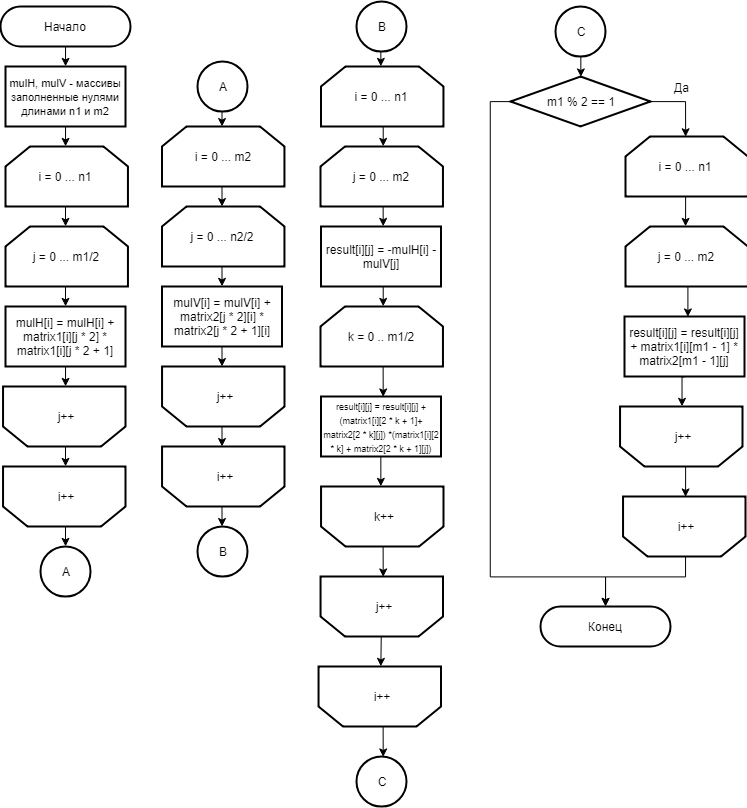
\includegraphics[scale=0.5]{BlockSchemeMult-Vin.png}
		
		Рисунок 1. Схема алгоритма Винограда.
	\end{center}

	\section*{Вывод}
	\addcontentsline{toc}{section}{Вывод}
	
	В данном разделе предсталена схема рассматриваемого в данной лабораторной работе алгоритма.
	
	\chapter{Технологическая часть}
	
	\section{Выбор ЯП}
	В качестве языка программирования был выбрал C++ \cite{2}, так как он позволяет реализовать задачу максимально комфортно.
	Для реализации многопоточности выбрана библиотека <threads> \cite{3}.
	
	\section{Замеры времени}
	Замер времени работы алгоритмов производился при помощи функций clock() из библиотеки time.h \cite{4}.
	
	\section{Генерация матриц для экспериментов}
	
	Все матрицы будут сгенерированы при помощи функции, создающей матрицу заданного размера, полностью заполненную единицами.
	
	\section{Листинг кода}
	
	\begin{center}
	Листинг 3.1. Реализация многопоточного умножения матриц методом Винограда.
	\end{center}
	\lstinputlisting[language=C++]{../code/lab_04/winmult.cpp}
	
	\section*{Вывод}
	\addcontentsline{toc}{chapter}{Вывод}
	
	В данном разделе обоснован выбор языка, описаны средства работы с многопоточностью, описан способ замера времени. Также реализован рассматриваемый алгоритм и представлен его литинг.
	
	\chapter{Эксперементальная часть}
	
	Исследуем работу алгоритма и сравним время выполнения при обработке матриц размером $ 100\times100,\dots, 1000\times1000$ и $ 101\times101,\dots, 1001\times1001$ с шагом 100 при обработке 1, 2, ... , 64 потоками. Время будем замерять в секундах.
	
	Эксперимент проводоился на следующей системе:
	\begin{enumerate}
		\item Intel(R) Core(TM) i7-3770K
		\item 8.00 ГБ ОЗУ
	\end{enumerate}
	
	\section{Сравнительный анализ времени работы алгоритма}
	
	\subsection{Четная размерность}
	
	В Таблице 1. - Таблице 7. представлены времена работы алгоритмов в зависимости от размерности при различном количестве потоков.
	~\\
	
	\begin{minipage}{0.5\textwidth}
		\begin{center}
			Таблица 1. Временя работы алгоритма при одном потоке.
			
			\begin{tabular}{|c c|}
				\hline
				Размер & Время (с) \\
				\hline
				100 & 0.014000\\
				\hline
				200 & 0.089000\\
				\hline
				300 & 0.295000\\
				\hline
				400 & 0.741000\\
				\hline
				500 & 1.506000\\
				\hline
				600 & 3.650000\\
				\hline
				700 & 5.656000\\
				\hline
				800 & 8.845000\\
				\hline
				900 & 13.468000\\
				\hline
				1000 & 21.052000\\
				\hline
			\end{tabular}
		\end{center}
	\end{minipage}
	\hfill
	\begin{minipage}{0.5\textwidth}
		\begin{center}
			Таблица 2. Временя работы алгоритма при двух потоках.
			
			\begin{tabular}{|c c|}
				\hline
				Размер & Время (с) \\
				\hline
				100 & 0.018000\\
				\hline
				200 & 0.047000\\
				\hline
				300 & 0.155000\\
				\hline
				400 & 0.384000\\
				\hline
				500 & 0.768000\\
				\hline
				600 & 1.398000\\
				\hline
				700 & 2.627000\\
				\hline
				800 & 3.768000\\
				\hline
				900 & 6.208000\\
				\hline
				1000 & 10.216000\\
				\hline
			\end{tabular}
			
			
		\end{center}
	\end{minipage}

	\begin{minipage}{0.5\textwidth}
		\begin{center}
			Таблица 3. Временя работы алгоритма при четырех потоках.
			
			\begin{tabular}{|c c|}
				\hline
				Размер & Время (с) \\
				\hline
				100 & 0.010000\\
				\hline
				200 & 0.027000\\
				\hline
				300 & 0.095000\\
				\hline
				400 & 0.225000\\
				\hline
				500 & 0.502000\\
				\hline
				600 & 0.783000\\
				\hline
				700 & 1.238000\\
				\hline
				800 & 2.041000\\
				\hline
				900 & 3.434000\\
				\hline
				1000 & 5.190000\\
				\hline
			\end{tabular}
		
			~\\
		
			Таблица 5. Временя работы алгоритма при шестнадцати потоках.
		
			\begin{tabular}{|c c|}
				\hline
				Размер & Время (с) \\
				\hline
				100 & 0.015000\\
				\hline
				200 & 0.031000\\
				\hline
				300 & 0.106000\\
				\hline
				400 & 0.232000\\
				\hline
				500 & 0.551000\\
				\hline
				600 & 0.944000\\
				\hline
				700 & 1.310000\\
				\hline
				800 & 1.884000\\
				\hline
				900 & 3.215000\\
				\hline
				1000 & 4.963000\\
				\hline
			\end{tabular}
		\end{center}
	\end{minipage}
	\hfill
	\begin{minipage}{0.5\textwidth}
		\begin{center}
			Таблица 4. Временя работы алгоритма при восьми потоках.
			
			\begin{tabular}{|c c|}
				\hline
				Размер & Время (с) \\
				\hline
				100 & 0.010000\\
				\hline
				200 & 0.043000\\
				\hline
				300 & 0.086000\\
				\hline
				400 & 0.204000\\
				\hline
				500 & 0.464000\\
				\hline
				600 & 0.717000\\
				\hline
				700 & 1.174000\\
				\hline
				800 & 1.805000\\
				\hline
				900 & 2.983000\\
				\hline
				1000 & 4.321000\\
				\hline
			\end{tabular}
		
		~\\
		
			Таблица 6. Временя работы алгоритма при тридцати двух потоках.
		
			\begin{tabular}{|c c|}
				\hline
				Размер & Время (с) \\
				\hline
				100 & 0.027000\\
				\hline
				200 & 0.040000\\
				\hline
				300 & 0.109000\\
				\hline
				400 & 0.264000\\
				\hline
				500 & 0.529000\\
				\hline
				600 & 0.991000\\
				\hline
				700 & 1.672000\\
				\hline
				800 & 2.211000\\
				\hline
				900 & 3.180000\\
				\hline
				1000 & 5.12000\\
				\hline
			\end{tabular}
		\end{center}
	\end{minipage}
		
	\begin{center}
		Таблица 7. Временя работы алгоритма при шестидесяти четырех потоках.
		
		\begin{tabular}{|c c|}
			\hline
			Размер & Время (с) \\
			\hline
			100 & 0.052000\\
			\hline
			200 & 0.054000\\
			\hline
			300 & 0.127000\\
			\hline
			400 & 0.231000\\
			\hline
			500 & 0.584000\\
			\hline
			600 & 0.853000\\
			\hline
			700 & 1.726000\\
			\hline
			800 & 2.218000\\
			\hline
			900 & 2.995000\\
			\hline
			1000 & 4.856000\\
			\hline
		\end{tabular}
	\end{center}
	
	
	
		\begin{center}
			\begin{tikzpicture}
			\begin{axis}[
			axis lines = left,
			xlabel = $\texttt{Размер}$,
			ylabel = $\texttt{Время (сек.)}$,
			legend pos=outer north east,
			ymajorgrids=true
			]
			
			\addplot[color=green] table[x index=0, y index=1] {info_1_ev.dat};
			\addplot[color=blue] table[x index=0, y index=1] {info_2_ev.dat};
			\addplot[color=red] table[x index=0, y index=1] {info_4_ev.dat};
			
			\addlegendentry{1 поток}
			\addlegendentry{2 потока}
			\addlegendentry{4 потока}
			\end{axis}
			\end{tikzpicture}
			
			Рисунок 1. График времен работы алгоритма при 1, 2, 4 потоках.
		\end{center}
	
		\begin{center}
			\begin{tikzpicture}
			\begin{axis}[
			axis lines = left,
			xlabel = $\texttt{Размер}$,
			ylabel = $\texttt{Время (сек.)}$,
			legend pos=outer north east,
			ymajorgrids=true
			]
			
			\addplot[color=green] table[x index=0, y index=1] {info_8_ev.dat};
			\addplot[color=blue] table[x index=0, y index=1] {info_16_ev.dat};
			\addplot[color=red] table[x index=0, y index=1] {info_32_ev.dat};
			\addplot[color=purple] table[x index=0, y index=1] {info_64_ev.dat};
			
			\addlegendentry{8 потоков}
			\addlegendentry{16 потоков}
			\addlegendentry{32 потока}
			\addlegendentry{64 потока}
			\end{axis}
			\end{tikzpicture}
			
			Рисунок 2. График времен работы алгоритма при 8, 16, 32, 64 потоках.
		\end{center}
	
		\begin{center}
			\begin{tikzpicture}
			\begin{axis}[
			axis lines = left,
			xlabel = $\texttt{Размер}$,
			ylabel = $\texttt{Время (сек.)}$,
			legend pos=outer north east,
			ymajorgrids=true
			]
			
			\addplot[color=green] table[x index=0, y index=1] {info_4_ev.dat};
			\addplot[color=blue] table[x index=0, y index=1] {info_8_ev.dat};
			\addplot[color=red] table[x index=0, y index=1] {info_32_ev.dat};
			
			\addlegendentry{4 потока}
			\addlegendentry{8 потоков}
			\addlegendentry{32 потока}
			\end{axis}
			\end{tikzpicture}
			
			Рисунок 3. График времен работы алгоритма при 4, 8, 32 потоках.
		\end{center}
	\newpage
	\textbf{Вывод по данному случаю:}
	
	Из Рисунка 3. и Рисунка 2. видно, что при восьми потоках время работы данного алгоритма наименьшее.
	
	Время работы алгоритма при восьми потоках на матрицах размера $1000$x$1000$ составляет 4.32 с, при $800$x$800$ - 1.8 с.
	
	\subsection{Нечетная размерность}
	
	В Таблице 8. - Таблице 14. представлены времена работы алгоритмов в зависимости от размерности при различном количестве потоков.
	~\\
	
	\begin{minipage}{0.5\textwidth}
		\begin{center}
			Таблица 8. Временя работы алгоритма при одном потоке.
			
			\begin{tabular}{|c c|}
				\hline
				Размер & Время (с) \\
				\hline
				101 & 0.022000\\
				\hline
				201 & 0.092000\\
				\hline
				301 & 0.324000\\
				\hline
				401 & 0.826000\\
				\hline
				501 & 1.752000\\
				\hline
				601 & 2.821000\\
				\hline
				701 & 4.847000\\
				\hline
				801 & 9.657000\\
				\hline
				901 & 13.795000\\
				\hline
				1001 & 21.118000\\
				\hline
			\end{tabular}
		\end{center}
	\end{minipage}
	\hfill
	\begin{minipage}{0.5\textwidth}
		\begin{center}
			Таблица 9. Временя работы алгоритма при двух потоках.
			
			\begin{tabular}{|c c|}
				\hline
				Размер & Время (с) \\
				\hline
				101 & 0.009000\\
				\hline
				201 & 0.062000\\
				\hline
				301 & 0.176000\\
				\hline
				401 & 0.429000\\
				\hline
				501 & 0.999000\\
				\hline
				601 & 1.783000\\
				\hline
				701 & 2.334000\\
				\hline
				801 & 3.616000\\
				\hline
				901 & 6.006000\\
				\hline
				1001 & 10.169000\\
				\hline
			\end{tabular}
			
			
		\end{center}
	\end{minipage}
	
	\begin{minipage}{0.5\textwidth}
		\begin{center}
			Таблица 10. Временя работы алгоритма при четырех потоках.
			
			\begin{tabular}{|c c|}
				\hline
				Размер & Время (с) \\
				\hline
				101 & 0.026000\\
				\hline
				201 & 0.051000\\
				\hline
				301 & 0.097000\\
				\hline
				401 & 0.248000\\
				\hline
				501 & 0.549000\\
				\hline
				601 & 0.915000\\
				\hline
				701 & 1.282000\\
				\hline
				801 & 1.911000\\
				\hline
				901 & 3.202000\\
				\hline
				1001 & 5.034000\\
				\hline
			\end{tabular}
			
			~\\
			
			Таблица 12. Временя работы алгоритма при шестнадцати потоках.
			
			\begin{tabular}{|c c|}
				\hline
				Размер & Время (с) \\
				\hline
				101 & 0.015000\\
				\hline
				201 & 0.035000\\
				\hline
				301 & 0.101000\\
				\hline
				401 & 0.226000\\
				\hline
				501 & 0.486000\\
				\hline
				601 & 0.793000\\
				\hline
				701 & 1.278000\\
				\hline
				801 & 1.790000\\
				\hline
				901 & 2.718000\\
				\hline
				1001 & 4.252000\\
				\hline
			\end{tabular}
		\end{center}
	\end{minipage}
	\hfill
	\begin{minipage}{0.5\textwidth}
		\begin{center}
			Таблица 11. Временя работы алгоритма при восьми потоках.
			
			\begin{tabular}{|c c|}
				\hline
				Размер & Время (с) \\
				\hline
				101 & 0.010000\\
				\hline
				201 & 0.029000\\
				\hline
				301 & 0.093000\\
				\hline
				401 & 0.217000\\
				\hline
				501 & 0.449000\\
				\hline
				601 & 0.781000\\
				\hline
				701 & 1.209000\\
				\hline
				801 & 1.912000\\
				\hline
				901 & 2.808000\\
				\hline
				1001 & 4.457000\\
				\hline
			\end{tabular}
			
			~\\
			
			Таблица 13. Временя работы алгоритма при тридцати двух потоках.
			
			\begin{tabular}{|c c|}
				\hline
				Размер & Время (с) \\
				\hline
				101 & 0.026000\\
				\hline
				201 & 0.040000\\
				\hline
				301 & 0.116000\\
				\hline
				401 & 0.269000\\
				\hline
				501 & 0.534000\\
				\hline
				601 & 0.934000\\
				\hline
				701 & 1.396000\\
				\hline
				801 & 1.809000\\
				\hline
				901 & 3.021000\\
				\hline
				1001 & 4.939000\\
				\hline
			\end{tabular}
		\end{center}
	\end{minipage}
	
	\begin{center}
		Таблица 14. Временя работы алгоритма при шестидесяти четырех потоках.
		
		\begin{tabular}{|c c|}
			\hline
			Размер & Время (с) \\
			\hline
			101 & 0.054000\\
			\hline
			201 & 0.056000\\
			\hline
			301 & 0.134000\\
			\hline
			401 & 0.263000\\
			\hline
			501 & 0.680000\\
			\hline
			601 & 0.934000\\
			\hline
			701 & 1.773000\\
			\hline
			801 & 2.347000\\
			\hline
			901 & 3.086000\\
			\hline
			1001 & 4.991000\\
			\hline
		\end{tabular}
	\end{center}
	
	
	
	\begin{center}
		\begin{tikzpicture}
		\begin{axis}[
		axis lines = left,
		xlabel = $\texttt{Размер}$,
		ylabel = $\texttt{Время (сек.)}$,
		legend pos=outer north east,
		ymajorgrids=true
		]
		
		\addplot[color=green] table[x index=0, y index=1] {info_1_ev.dat};
		\addplot[color=blue] table[x index=0, y index=1] {info_2_ev.dat};
		\addplot[color=red] table[x index=0, y index=1] {info_4_ev.dat};
		
		\addlegendentry{1 поток}
		\addlegendentry{2 потока}
		\addlegendentry{4 потока}
		\end{axis}
		\end{tikzpicture}
		
		Рисунок 4. График времен работы алгоритма при 1, 2, 4 потоках.
	\end{center}
	
	\begin{center}
		\begin{tikzpicture}
		\begin{axis}[
		axis lines = left,
		xlabel = $\texttt{Размер}$,
		ylabel = $\texttt{Время (сек.)}$,
		legend pos=outer north east,
		ymajorgrids=true
		]
		
		\addplot[color=green] table[x index=0, y index=1] {info_8_nv.dat};
		\addplot[color=blue] table[x index=0, y index=1] {info_16_nv.dat};
		\addplot[color=red] table[x index=0, y index=1] {info_32_nv.dat};
		\addplot[color=purple] table[x index=0, y index=1] {info_64_nv.dat};
		
		\addlegendentry{8 потоков}
		\addlegendentry{16 потоков}
		\addlegendentry{32 потока}
		\addlegendentry{64 потока}
		\end{axis}
		\end{tikzpicture}
		
		Рисунок 5. График времен работы алгоритма при 8, 16, 32, 64 потоках.
	\end{center}
	
	\begin{center}
		\begin{tikzpicture}
		\begin{axis}[
		axis lines = left,
		xlabel = $\texttt{Размер}$,
		ylabel = $\texttt{Время (сек.)}$,
		legend pos=outer north east,
		ymajorgrids=true
		]
		
		\addplot[color=green] table[x index=0, y index=1] {info_4_nv.dat};
		\addplot[color=blue] table[x index=0, y index=1] {info_8_nv.dat};
		\addplot[color=red] table[x index=0, y index=1] {info_32_nv.dat};
		
		\addlegendentry{4 потока}
		\addlegendentry{8 потоков}
		\addlegendentry{32 потока}
		\end{axis}
		\end{tikzpicture}
		
		Рисунок 6. График времен работы алгоритма при 4, 8, 32 потоках.
	\end{center}
	\newpage
	\textbf{Вывод по данному случаю:}
	
	Из Рисунка 5. и Рисунка 6. видно, что при восьми потоках время работы данного алгоритма наименьшее.
	
	Время работы алгоритма при восьми потоках на матрицах размера $1001$x$1001$ составляет 4.45 с, при $800$x$800$ - 1.91 с.
	
	\section*{Вывод}
	\addcontentsline{toc}{chapter}{Вывод}
	
	В данной главе проведет эксперимент по измерению времени работы рассматриваемого алгоритма в зависимости от количества потоков. Рассматривались матрицы четного и нечетного размера.
	
	В результате сделан вывод, что для матриц четного размера, также как и для матриц нечетного размера, наилучшая производительность достигается при количестве потоков равном восьми. При таком количестве потоков время умножения матриц $800$x$800$ равно 1.8 с, $801$x$801$ - 1.91 с, $1000$x$1000$ - 4.32с, $1001$x$1001$ - 4.45 с.
	
	При работе с одним потоком время умножения матриц $801$x$801$ в 5 раз больше, матриц $800$x$800$ в 7 раз больше, $1001$x$1001$ в 4.74 раза больше, $1000$x$1000$ в 4.73 раза больше.
	
	\chapter*{Заключение}
	\addcontentsline{toc}{chapter}{Заключение}
	
	В ходе выполнения данной лабораторной был работы реализован оптимизированный, при помощи распараллеливания вычислений, алгоритм Винограда. 
	
	Также проведено исследование поведения алгоритма при различном количестве потоков, на основании проведенного эксперимента. В этом эксперементе матрицы $100$x$100$, $200$x$200$, ... , $1000$x$1000$ и $101$x$101$, $201$x$201$, ... , $1001$x$1001$ перемножались сами с собой, при этом использовалось разное количество потоков (1, 2, 4, .. , 64).
	
	В результате этого исследования сделан вывод, что наилудшая производительность достигается при восьми потоках. При таком количестве потоков получилось ускорить время работы, по сравнению с одним потоком, в 5 раз для $801$x$801$, в 7 раз для $800$x$800$, в 4.74 раза для $1001$x$1001$ и в 4.73 раза для $1000$x$1000$.
	
	\bibliographystyle{utf8gost705u}
	\bibliography{lib} 
	
\end{document}